\title{CS 513 Assignment 5}
\author{Ruochen Lin}
\documentclass[11pt]{article}
\usepackage{amsmath,amsfonts,amssymb,amsthm}
\usepackage{mathtools}
\usepackage{commath}
\usepackage{setspace}
% \usepackage{algorithm,algorithmic}
\begin{document}
\maketitle
\section{}
\subsection{}
We start with LU-factorization first. We only need to know the number of negative eigenvalues on the diagonal of $U$ matrices after decomposition, so we only need to update the diagonal elements. If we denote the resulting upper triangular matrices from the LU decomposition of $A$ and $A-I$ as $U_0$ and $U_1$, the diagonal elements of $U_0$ are -1, 2 and 1.5, and the those of $U_1$ are -2, 0.5 and -1. Thus there is one eigenvalue of $A$ in $(0,1)$.\\[0.3cm]
Now, let's calculate the determinants of the principal minors of $A$ and $A-I$ to achieve the same goal. The determinants of the principal minors of $A$ are -1, -2, and -5, and those of $A-I$ are -2, -1, and 1. Considering the implicit 1 at the beginning of the sequence, the number of negative eigenvalues of $A$ and $A-I$ are 1 and 2. Thus, there is 1 eigenvalue of $A$ in the interval of $(0,1)$.

\subsection{}
In the LU approach, we calculated $1 - 1^2/(-1) = 2$ and $2 - 1^2/2 = 1.5$ for $A$ and $0-1^2/(-2) = 0.5$ and $1-1^2/0.5 = -1$ for $A-I$: a total of 2 multiplications and 2 divisions were carried out for each matrix. The formula used to update the diagonal elements is $U_{k,k} = A_{k,k} - A_{k,k-1}^2/U_{k-1,k-1}.$ In general, for a $m\times m$ tridiagonal matrix, $m-1$ multiplications and $m-1$ divisions needs to be carried out.\\[0.3cm]
When calculating the determinants, if we set $d(0)=1$ and $d(1)=A_{1,1}$, the recurrent formula is $d(k) = A_{k,k}*d(k-1)-A_{k,k-1}^2*d(k-2)$. For $k=2,\cdots,m$, we use the recurrent formula to calculate the determinants of the corresponding minors: a total of $3(m-1)$ multiplications are needed.\\[0.3cm]
If we deem the cost of division as the same as that of multiplication, we might come to the conclusion that LU-factorization is a better algorithm. However, on most machines, floating-point division, which can cost as many as more than 10 clock cycles, is about 3--5 times slower than multiplication; thus, we expect the determinant approach to have better performance. In addition, doing LU-factorization without pivotting always risks encountering zero or small diagonal entries: another point for determinants!
\subsection{}
Figure 1 is a plot of time consumed to find the number of eigenvalues between 0 and 1 for symmetric 
Figure 1 shows that both methods generally have linear complexity for random symmetric tridiagonal matrices. The determinant method is more efficient, compared to LU-factorization, which agrees with our analysis above.
\begin{figure}[t]
\centering
{
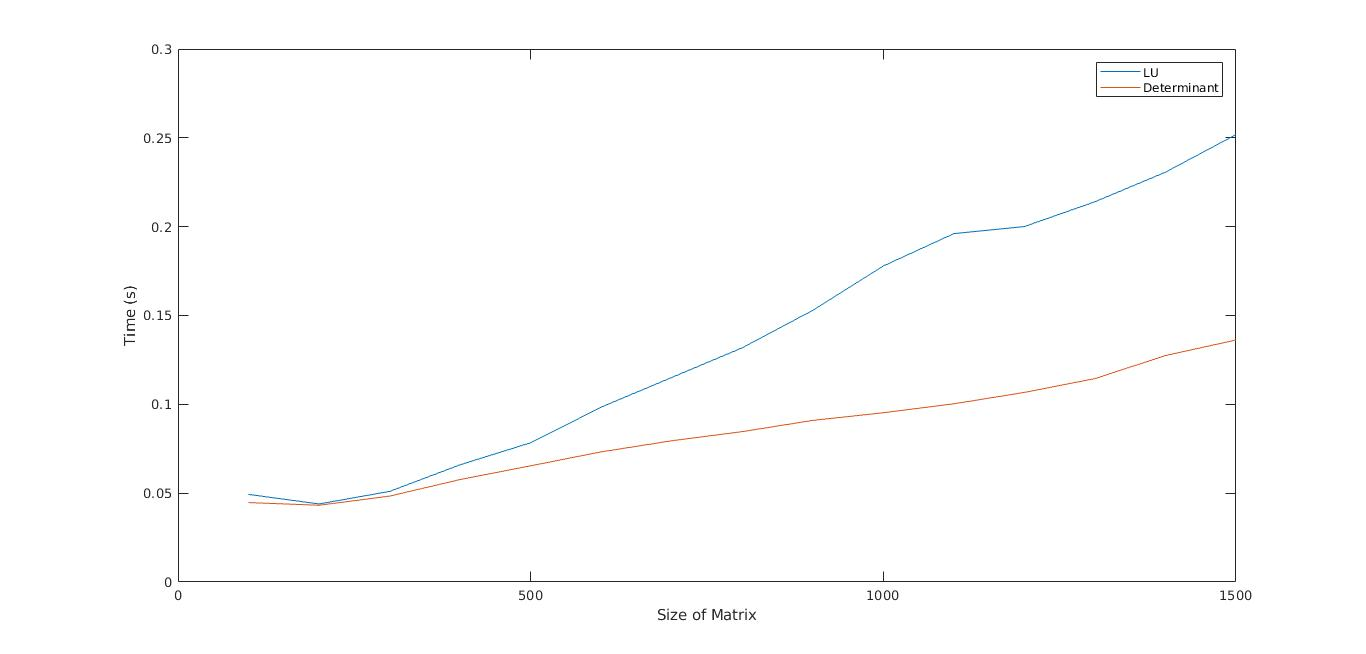
\includegraphics[width=10cm]{matlab/prob1.jpg}
\caption{plot of time consumed to find the number of eigenvalues between 0 and 1 for symmetric tridiagonal matrices of different sizes. The time shown is the total of operating on 1,000 matrices of each size.}
}
\end{figure}
\pagebreak
\section{}
\subsection{}
The cardinality of $\sigma(A)$ is $n$, because in each of the pairwise disjoint disks there is one (and only one) eigenvalue of $A$, which add up to give $n$ distinct eigenvalues. In addition, for each of the eigenvalues, both the corresponding algebraic and geometric multiplicity is $1$.

\subsection{}
The proposition is true, because for each of the eigenvalues of $A$, the algebraic multiplicity is equal to geometric multiplicity, which is a sufficient (and necessary) condition for $A$ to be diagonalizable.

\subsection{}
The claim is correct, and we can prove it by contradiction: If the imaginary part of an eigenvalue of a real matrix $A$ is not zero, namely $Av=\lambda v,\,\,\lambda =x+iy,\,\,y\neq0$, then we can take the complex conjugate of the equation to write $A\bar v = \bar\lambda\bar v$, namely $\bar\lambda$ will also be an eigenvalue of $A$. Since all of the Gershgorin disks of $A$ are centered on the real axis, if $\lambda=x+iy$ is in one of the disks, $\bar\lambda=x-iy$ will also be in the same disk. However, we know from preceeding discusions that in each of the Gershgorin disks there can be only one eigenvalue of $A$; hence we know that all of the eigenvalues of $A$ must be real.

\subsection{}
This is not true. The following is a counterexample: with a simple matrix whose Gershgorin disks are obvious disjoint:
\begin{equation}\begin{split} 
A = \begin{bmatrix}1&0\\0&-1 \end{bmatrix}, 
\end{split}\nonumber\end{equation}
and the input vector $x = \begin{bmatrix} 1&1\end{bmatrix}^T $, the sequence $\{A^nx\}_{n=1}^{\infty}$ oscillates back and forth between $\begin{bmatrix} 1&1\end{bmatrix}^T $ and $\begin{bmatrix} 1 & -1\end{bmatrix} $, which clearly does not converge.

\section{}

\section{}
\subsection{}
Answer: the diagonal and first and second superdiagonal entries of $R$ are potentially non-zero, and $Q$ is tridiagonal. The explanation is the following:\\[0.3cm]
Because $A$ is symmetric tridiagonal, \textit{i.e.} 
\begin{equation}\begin{split} 
A = \begin{bmatrix} 
a & b\\
b & c & d\\
& d & \ddots & \ddots\\
& & \ddots & x  & y \\
& & & y & z
\end{bmatrix},
\end{split}\nonumber\end{equation} 
when we're eliminating the subdiagonal entries of $A$ with Householders, $H_k$ needs only to alter the $k$th and $k+1$th rows. As a result, in the region above the diagonal, only the $(k,k+2)$ entry risks becoming nonzero from zero in the $k$th step. After $m-1$ steps, the only entries in $R$ that can be nonzero are ones on the diagonal, first superdiagonal and second superdiagonal. \\[0.3cm]
$Q=\prod_{k=1}^{m-1}H_k$ is the same as the resulting matrix after applying the operations, as detailed above, on the identity matrix: in each step nonzero elements are introduced in sub- and super-diagonal positions. After $m-1$ steps, it's obvious that $Q$ is tridiagonal.
\subsection{}
Because $A = QR = H_{m-1}H_{m-2}\cdots H_2 H_1R$, $RQ$ can be written as 
\begin{equation}\begin{split} 
RQ = RH_{m-1}\cdots H_1 \\
\end{split}\nonumber\end{equation}
The effect of $H_{m-1}$ on $R$ is `messing up' the last two columns while leaving other columns unchanged. Thus, in the lower triangular part of $RH_{m-1}$, the only nonzero entry is $(RH_{m-1})_{m, m-1}$. Similarly, the effect of $H_{m-2}$ on $RH_{m-1}$ is altering the $m-1$th and $m-2$th columns while keeping others intact\footnote{For a general $H_{m-2}$ operated from the right, the last three columns will be altered, and after $m-1$ operations the resulting matrix is no Hessenberg. However, since we started with a triadiagonal matrix in QR factorization, the $k$th Householder need only to change the $k$th and $k+1$th rows when operating from the left (or columns from the right); hence we have this nice property.}, and the only nonzero entries below diagonal now are at $(m,m-1)$ and $(m-1,m-2)$. After $m-1$ operations of Householder matrices from the right, all of the subdiagonal entries will potentially be nonzero, and the resulting matrix, $RQ$, is a Hessenberg matrix.\\[0.3cm]
In addition, we can write $R$ as 
\begin{equation}\begin{split} 
R = Q'A = H_{m-1}\cdots H_1A,
\end{split}\nonumber\end{equation} 
so that $RQ=Q'AQ$. Because $A$ is symmetric, $Q'AQ$ must be symmetric as well. Thus, $RQ$ is a symmetric Henssenberg matrix, which is tridiagonal.
 
\end{document}
